% -*- root: ../../main.tex -*-
\section{Audio Manager}
\label{sec:audio_manager_design}
I videogiochi richiedono in generale il lanciano di un elevato numero di suoni per partita, spesso questi effetti sonori sono legati a eventi o a interazioni con la GUI del gioco.

Anche le canzoni ricoprono spesso un ruolo di sottofondo, anche se intervallate con minor frequenza.

L'elevata frequenza di eventi ha portato allo sviluppo di un \textbf{Agente}, inteso come un flusso di controllo separato che ha il compito di gestire e manipolare internamente tutte musiche e gli effetti sonori che gli vengono inviati.


Il \textbf{SoundAgent} utilizza una coda di eventi per tracciare tutte le azioni che deve effettuare, gli utilizzatori possono infatti accodare eventi esternamente, senza inquinare l'operatività del proprio flusso di controllo.

Un flusso di controllo separato consente di disaccoppiare al massimo il carico di lavoro, il continuo lanciare di musiche e suoni può essere deleterio per le prestazioni, è infatti oneroso lanciare un suono specie se ripetutamente ad intervalli irregolari.

Tale carico non deve gravare nella logica principale del programma né tantomeno sulla \textbf{view}, il carico necessario per l'accodamento di un evento è molto minore, ripartendo così il grosso del lavoro sul \textbf{Thread} dell'SoundAgent.

\begin{figure}[H]
	\centering
	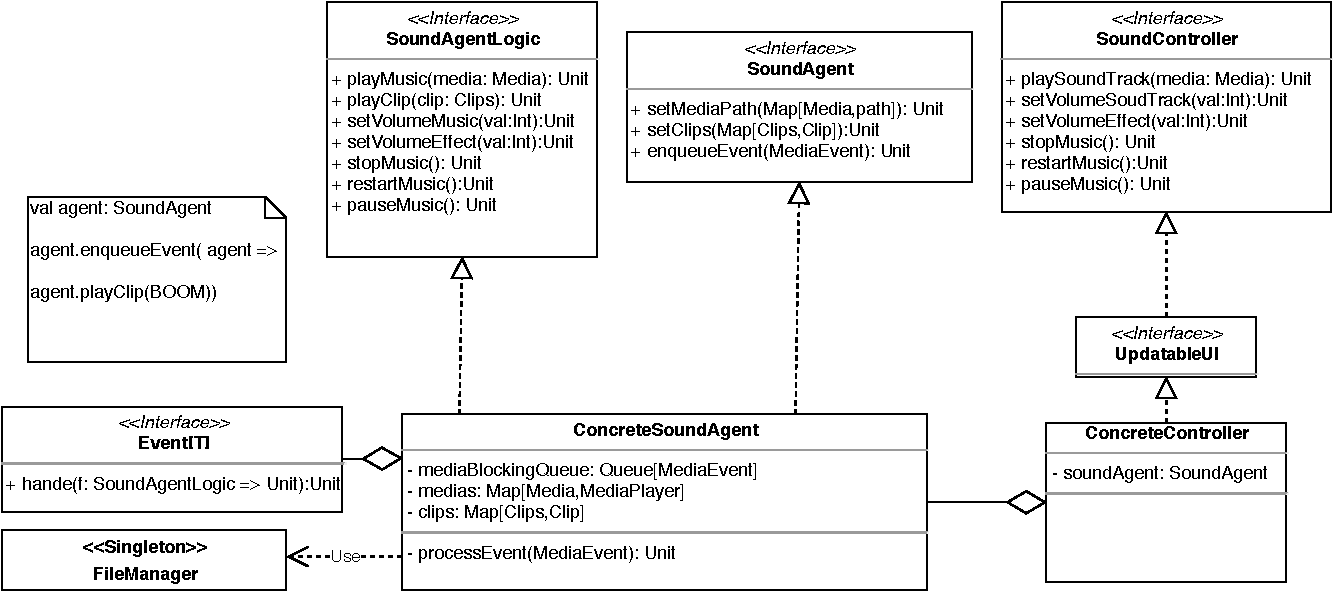
\includegraphics[width=0.99\columnwidth]{drawio/audioAgent/audioAgent.pdf}
	\caption{Diagramma di classe rappresentante la struttura del SoundAgent.}
	\label{fig:AudioAgent}
\end{figure}

Un solo SoundAgent è in grado di riprodurre una grossa quantità di clip, ciò nonostante è possibile istanziarne più di uno, questo per non limitare il numero di suoni, è inoltre possibile creare SoundAgent specifici.

Un eventuale utilizzatore tramite il pattern \textbf{Strategy} può schedulare un evento all'agent, questo grazie all'interfaccia \textbf{Sealed SoundAgentLogic}
e alla coda di \textbf{Event}.

Questo consente di evitare l'utilizzo di \textbf{if} all'interno dell'agente, rendendo l'esecuzione più performante e il codice più snello.